\section{Morphogenesis and Replication of 2D Patterns}
\label{sec:prev_work}
The first class of problems CA-NEAT was tested on was \textit{morphology problems}, in the form of the two related problem of morphogenesis and replication.
The patterns used in these experiments are shown in Figure \ref{fig:patterns}

\begin{figure*}
\centering
\begin{subfigure}[b]{.20\textwidth}
\centering
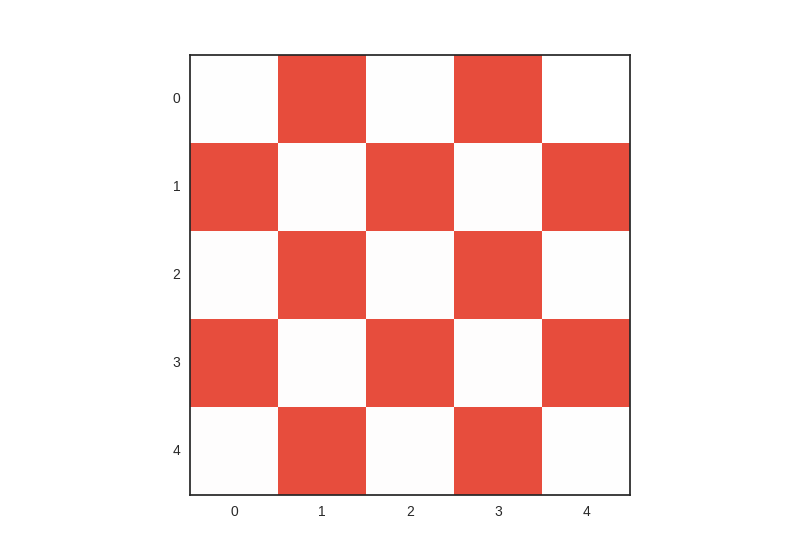
\includegraphics[width=\textwidth]{fig/mosaic}
\caption{5x5 "Mosaic"}
\label{fig:mosaic_pattern}
\end{subfigure}%
\begin{subfigure}[b]{.20\textwidth}
\centering
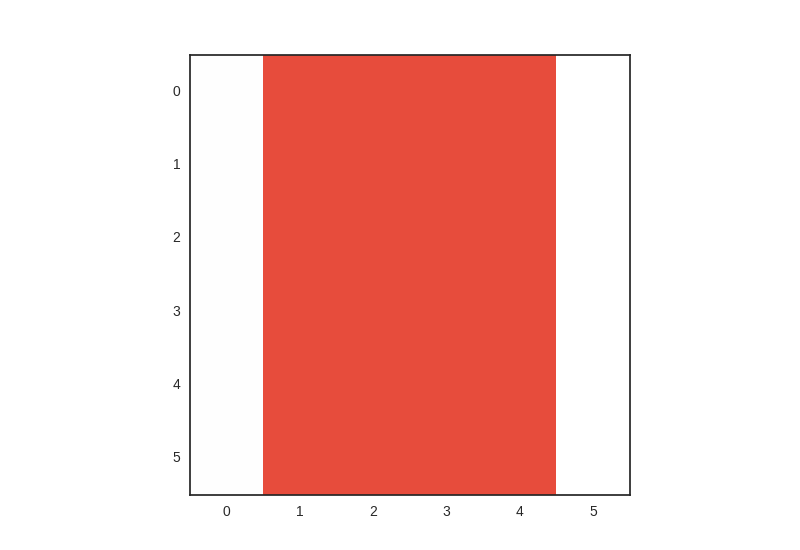
\includegraphics[width=\textwidth]{fig/border}
\caption{6x6 "Border"}
\end{subfigure}%
\begin{subfigure}[b]{.20\textwidth}
\centering
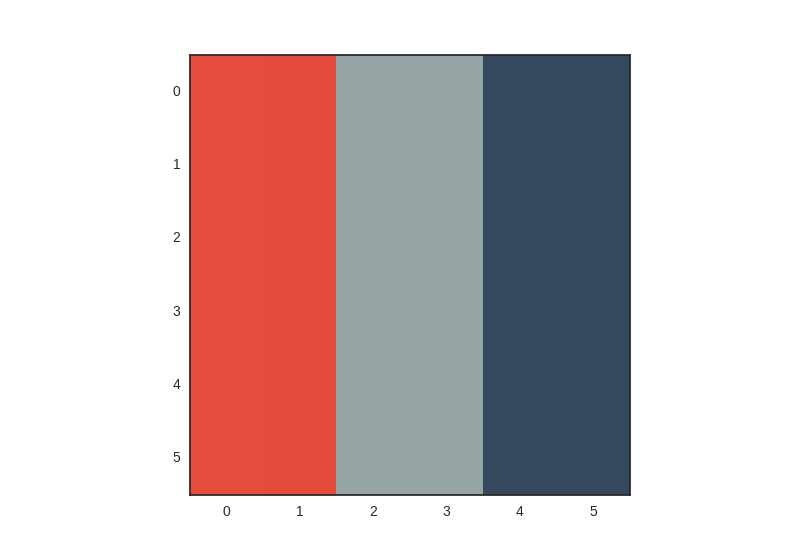
\includegraphics[width=\textwidth]{fig/tricolor}
\caption{6x6 "Tricolor"}
\end{subfigure}%
\begin{subfigure}[b]{.20\textwidth}
\centering
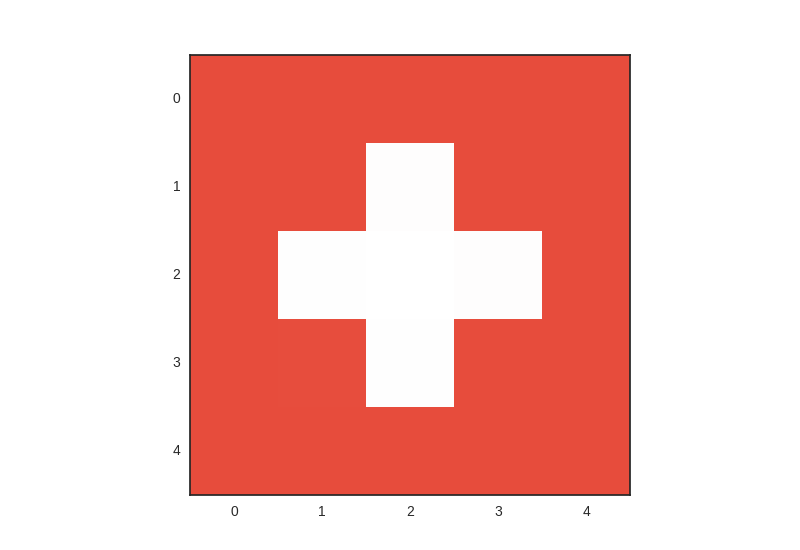
\includegraphics[width=\textwidth]{fig/swiss}
\caption{5x5 "Swiss"}
\end{subfigure}%
\begin{subfigure}[b]{.20\textwidth}
\centering
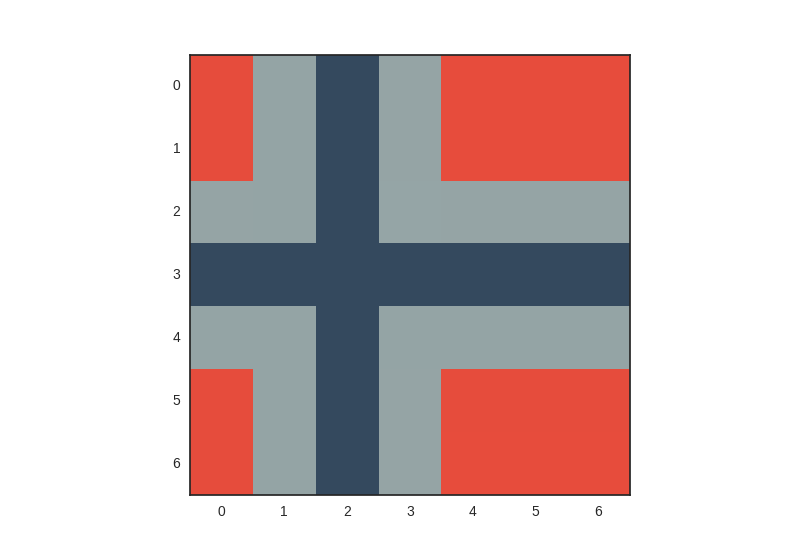
\includegraphics[width=\textwidth]{fig/nordic}
\caption{7x7 "Nordic"}
\end{subfigure}%

\caption{Patterns being investigated for morphogenesis and replication.}
\label{fig:patterns}
\end{figure*}

These are the same problems and patterns as studied in \cite{nichele2014evolutionary}, which used an instruction-based encoding and also tested table-based encoding for comparison.
This allowed the results of \cite{nichele2014evolutionary} to act as a benchmark for testing the CA-NEAT framework during development,
and to make comparisons between the results for analysis.

The experiments in this section were performed and analyzed in the specialization project leading up to this thesis project.
The report from the specialization project was further refined with co-authors Stefano Nichele, Gunnar Tufte and Sebastian Risi to a paper which at the time of writing has been accepted but not yet published in the IEEE Transactions on Cognitive and Developmental Systems.
TODO does mentioning the above go somewhere else?

\subsection{Morphogenesis problems}
\label{sec:morph_problems}
In CA terms, morphogenesis is the construction of a (more) complex pattern from a simple "seed" pattern.
The biological analogy and inspiration is \textit{embryonic development},
with the seed pattern also sometimes called a \textit{zygote}.
Figure \ref{fig:seed} shows the seed patterns used in these experiments.

\begin{figure}
\centering
\begin{subfigure}[b]{.30\columnwidth}
\centering
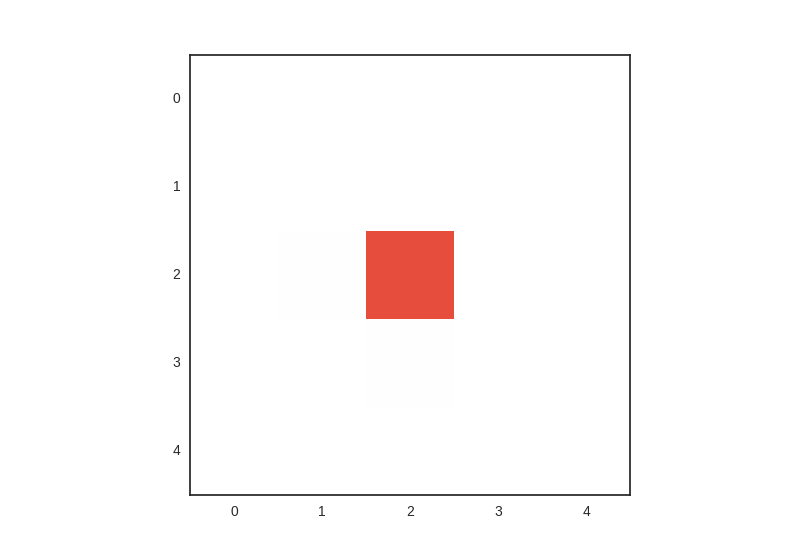
\includegraphics[width=\columnwidth]{fig/seed_5x5}
\caption{5x5}
\end{subfigure}%
\begin{subfigure}[b]{.30\columnwidth}
\centering
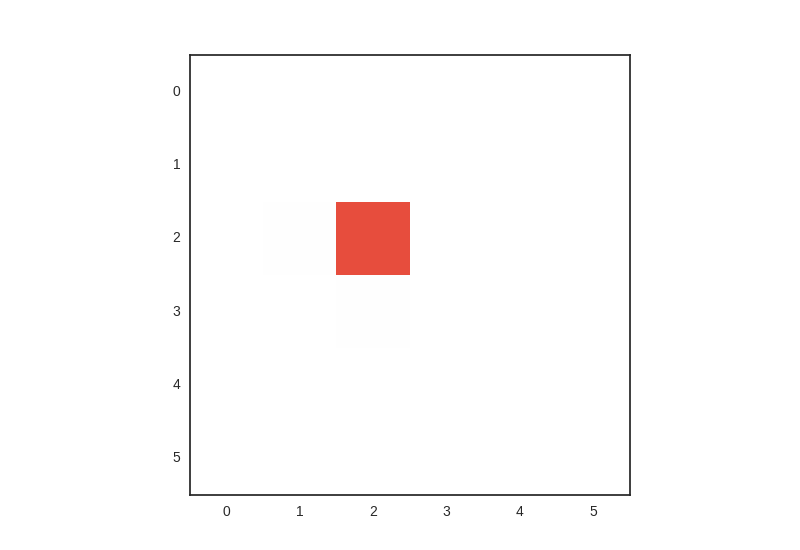
\includegraphics[width=\columnwidth]{fig/seed_6x6}
\caption{6x6}
\end{subfigure}%
\begin{subfigure}[b]{.30\columnwidth}
\centering
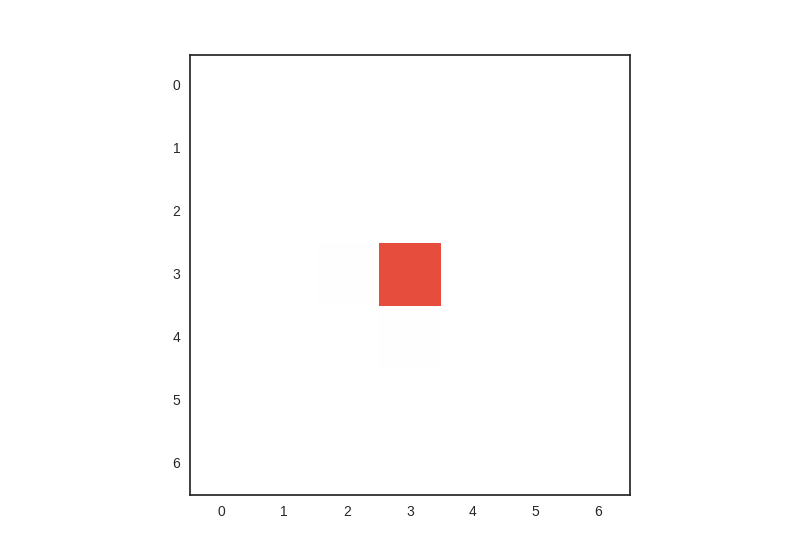
\includegraphics[width=\columnwidth]{fig/seed_7x7}
\caption{7x7}
\end{subfigure}%

\caption
[
    Seed patterns for morphogenesis.
]
{
    Seed patterns for morphogenesis.
    For the 6x6 patterns there is no central cell, so the seed is not symmetric.}
\label{fig:seed}
\end{figure}

The fitness evaluation function used in the morphogenesis experiments consists of the following steps:

\begin{enumerate}
    \item Develop seed pattern for 30 iterations
    \item For each stage
        \begin{enumerate}
            \item Compare cell by cell with  target pattern
            \item Calculate ratio of correct out of total cells
        \end{enumerate}
    \item Pick the highest of the values from step 2
    \item Use function \eqref{eq:redistribute} with value from step 3 as x
\end{enumerate}

\begin{equation}
    \label{eq:redistribute}
    f(x) = x * \frac{e^{5*x}}{e^{5}}
\end{equation}

In cases such as the "Mosaic" pattern (Figure \ref{fig:mosaic_pattern}), a completely dead CA (all cells in the quiescent state) would have a "correct cell" ratio of $0.52$.
Function \eqref{eq:redistribute} is used to reduce the score for such cases, while ensuring that $f(1.0) = 1.0$.

Because every iteration of the CA is counted equally and separately,
the fitness evaluation does not care if the CA becomes stable, enters a cycle, or neither within the 30 allotted iterations.
If the target pattern occurs at any point, that is enough to get a perfect score.

\subsection{Replication problems}
In a CA replication problem, the initial state has some complex pattern present.
The goal is to produce multiple copies of this initial patterns within the allotted time.
The biological analogy of this is cell division and asexual (clonal) reproduction.
For the replication problem the seed pattern is thus one copy of the target pattern in a larger grid.

The fitness evaluation for a replication phenotype is as follows:

\begin{enumerate}
    \item Develop seed pattern for 30 iterations
    \item For each stage
        \begin{enumerate}
            \item For each region of target pattern size
            \begin{enumerate}
                \item Compare cell by cell with  target pattern
                \item Calculate ratio of correct out of total cells
            \end{enumerate}
            \item Pick the highest 3 values from (a)
            \item Multiply any value less than $1.0$ by a penalty factor of $0.9$
            \item Calculate mean of three values
        \end{enumerate}
    \item Pick the highest value from stage (2)
\end{enumerate}

In this case the number of replicas sought is three.
There is no further contribution to the score if there are more than three perfect replicas.
But it follows logically that if one instance can be duplicated once, then each of the duplicates should be able to duplicate again, leading to exponential growth if time and space is not bounded.
Once again a penalty is applied, this time to penalize the contribution from any imperfect replica pattern, hopefully driving the selection pressure towards perfect replication.

Compared to the evaluation of morphogenesis of the same pattern, the replication evaluation is much more computationally expensive.
Therefore it will always take longer to collect results for a replication problem than the same-pattern morphogenesis problem.

\subsection{Cellular Model}
For both morphology problem categories a 2D CA model is used.
For the morphogenesis problem the grid is of fixed size with toroidal border conditions.
For the replication problem the grid is automatically expanding to accommodate growth in any direction.
In theory this means an infinite grid, but since the CA may only iterate 30 times, there is a practical limit to how large it may grow.
For both problem types the Von Neumann neighborhood (Figure \ref{fig:neighborhoods_vn}) is used.

\subsection{Results}
\begin{table*}[h]
    \centering
    \caption[Summary of results of morphology experiments]{
Summary of results.
The metrics shown are the success rate and the mean number of generations until a solution is found, with standard deviation also shown.
In the case of 100\% success rate, the number of generations column shows how many generations it took until the final solution was found.
In the case of less than 100\% success rate, the column shows how many generations were run until the experiment was stopped.
}
\begin{tabular}{lrrrr}
\hline
 Problem              &   Success rate \% &   Mean gens. &   $\sigma$ gens. &   Gens. until stop \\
\hline
Mosaic morphogenesis      &              100 &                1.2 &                 0.4 &                        2 \\
Border morphogenesis      &                1 &              270   &                 0   &                      509 \\
Tricolor morphogenesis    &              100 &               56.5 &               228.8 &                     2189 \\
Swiss morphogenesis       &               76 &              147.7 &               158.9 &                      600 \\
Mosaic replication        &              100 &                4.2 &                10.6 &                       99 \\
Swiss replication         &              100 &                7.7 &                 5   &                       20 \\
Tricolor replication      &               55 &               55.8 &                52.6 &                      200 \\
Nordic replication        &               0  &                  - &                   - &                      200 \\
\hline
\end{tabular}
\label{tbl:results}
\end{table*}

\begin{table}
    \centering
    \caption{Success rate at morphology problems for table-based, instruction-based and CA-NEAT transition functions found by GA.}
    \begin{tabular}{llll}
    \hline
    Problem                & Table-based & Instruction-based & CA-NEAT \\ \hline
    Mosaic morphogenesis   & 55\%        & 98\%              & 100\%   \\
    Swiss morphogenesis    & 23\%        & 100\%             & 76\%    \\
    Border morphogenesis   & 69\%        & 98\%              & 1\%     \\
    Tricolor morphogenesis & 19\%        & 46\%              & 100\%   \\
    Mosaic replication     & 85\%        & 100\%             & 100\%   \\
    Swiss replication      & 1\%         & 100\%             & 100\%   \\
    Tricolor replication   & 8\%         & 100\%             & 45\%    \\
    Nordic replication     & 0\%         & 100\%             & 0\%     \\ \hline
    \end{tabular}
\end{table}

\begin{figure}[t]
\centering
\begin{subfigure}[t]{.45\columnwidth}
\centering
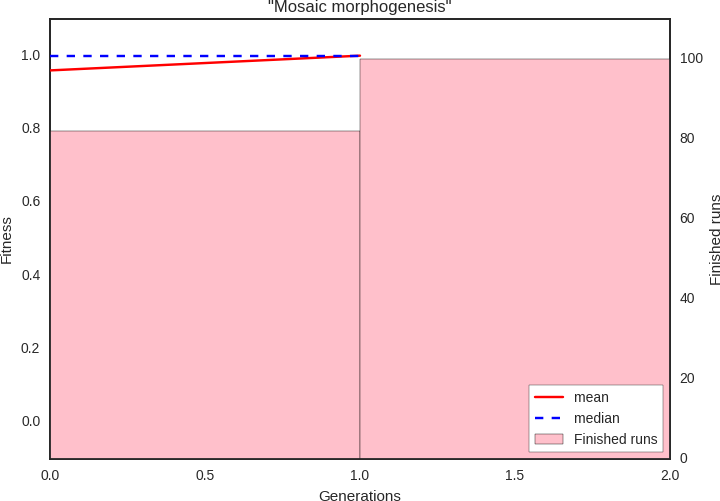
\includegraphics[width=\columnwidth]{fig/generate_mosaic_results}
\caption{Mosaic pattern morphogenesis, all generations.}
\label{fig:generate_mosaic_results}
\end{subfigure}
\begin{subfigure}[t]{.45\columnwidth}
\centering
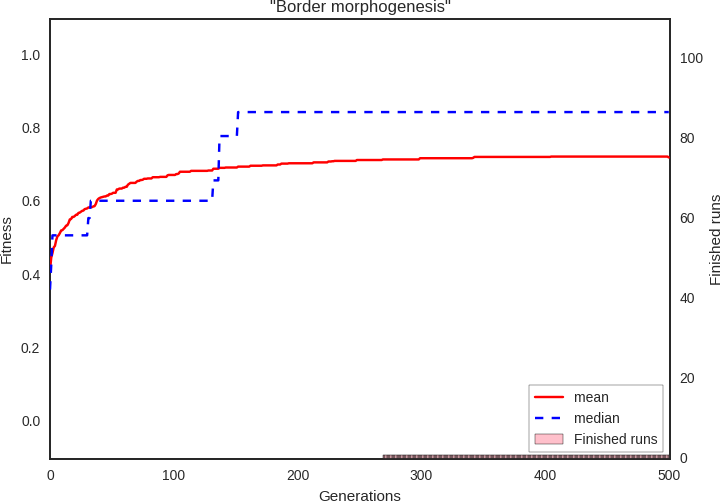
\includegraphics[width=\columnwidth]{fig/generate_border_results}
\caption{Border pattern morphogenesis, 500 first generations.
%The value where the median stabilizes represents the fitness for a solution with one wrong cell.
}
\label{fig:generate_border_results}
\end{subfigure}
\begin{subfigure}[t]{.45\columnwidth}
\centering
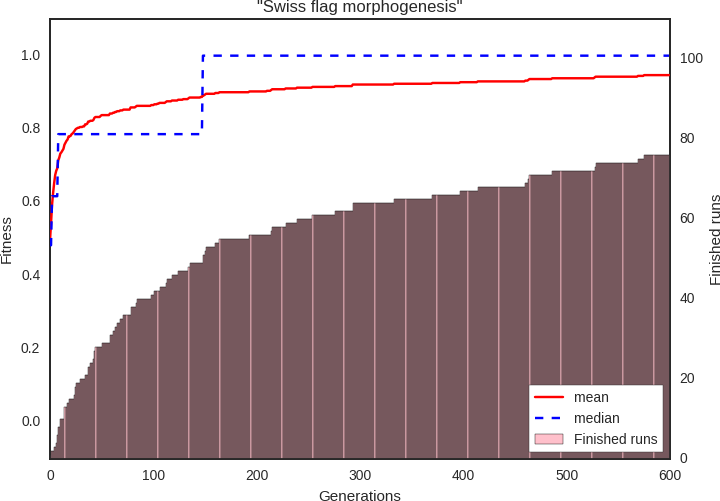
\includegraphics[width=\columnwidth]{fig/generate_swiss_results}
\caption{Swiss flag pattern morphogenesis, 600 first generations.}
\label{fig:generate_swiss_results}
\end{subfigure}
\begin{subfigure}[t]{.45\columnwidth}
\centering
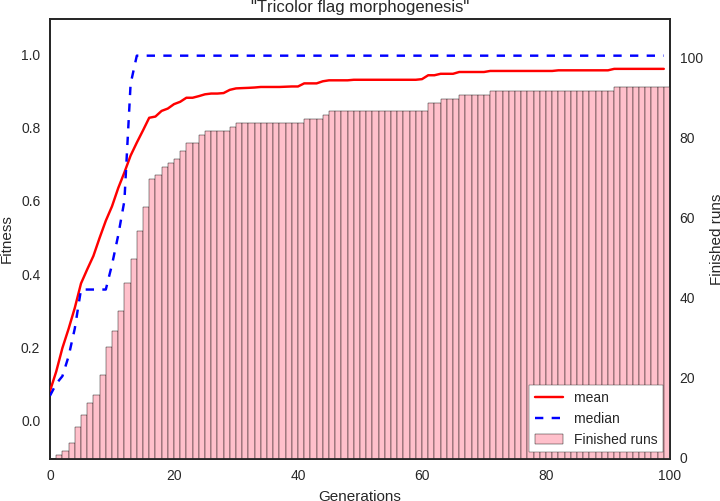
\includegraphics[width=\columnwidth]{fig/generate_tricolor_results}
\caption{Tricolor flag pattern morphogenesis, 100 first generations.}
\label{fig:generate_tricolor_results}
\end{subfigure}
\caption{
    Success rate (cumulative histogram) of the morphogenesis experiments.
    Also shows the mean and median of the max fitness in each run.
    }
\label{fig:morphogenesis_results}
\end{figure}

\begin{figure}[t]
\centering
\begin{subfigure}[t]{.45\columnwidth}
\centering
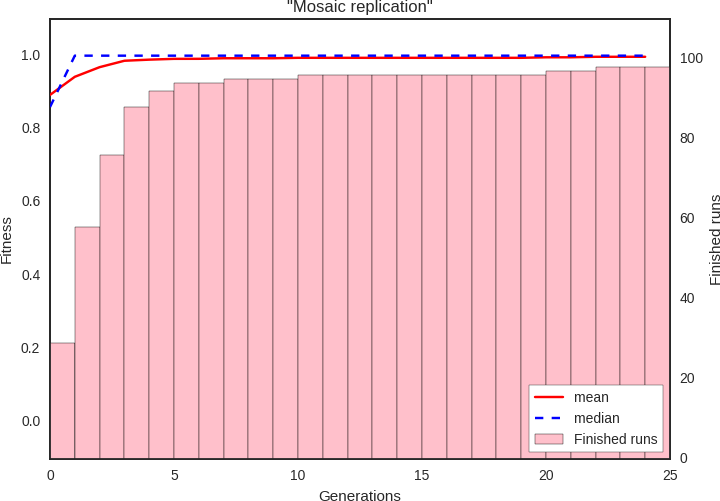
\includegraphics[width=\columnwidth]{fig/replicate_mosaic_results}
\caption{Mosaic pattern replication, 25 first generations.}
\label{fig:replicate_mosaic_results}
\end{subfigure}
\begin{subfigure}[t]{.45\columnwidth}
\centering
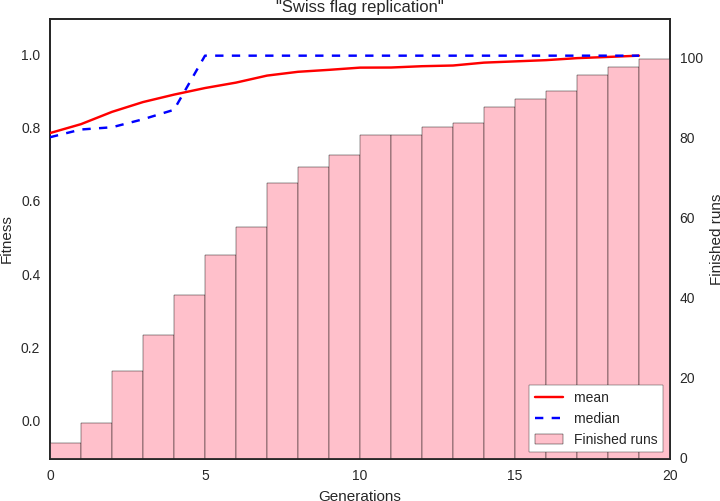
\includegraphics[width=\columnwidth]{fig/replicate_swiss_results}
\caption{Swiss flag pattern replication, all generations.}
\label{fig:replicate_swiss_results}
\end{subfigure}
\begin{subfigure}[t]{.45\columnwidth}
\centering
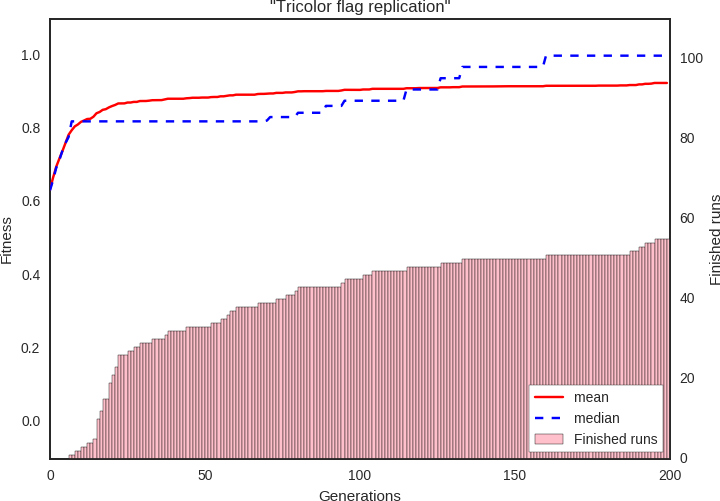
\includegraphics[width=\columnwidth]{fig/replicate_tricolor_results}
\caption{Tricolor flag pattern replication, 200 first generations.}
\label{fig:replicate_tricolor_results}
\end{subfigure}
\begin{subfigure}[t]{.45\columnwidth}
\centering
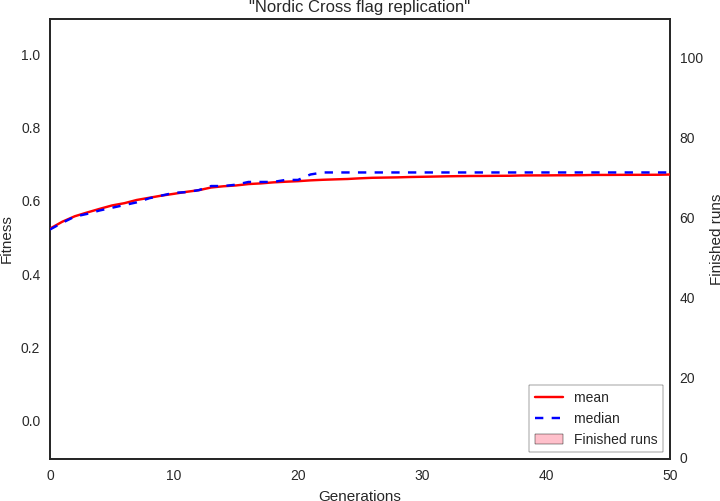
\includegraphics[width=\columnwidth]{fig/replicate_nordic_results}
\caption{Nordic cross pattern replication, 50 first generations.
%Further generations up to 200 did not have any significant change in the mean or median lines.
}
\label{fig:replicate_nordic_results}
\end{subfigure}
\caption{TODO}
\label{fig:replication_results}
\end{figure}

The results of the experiments were varied, with some problems being easily solved with CA-NEAT, some being slowly solved, and some not being consistently solved at all.
Table \ref{tbl:results} summarizes the results in terms of success rate and generations of evolution.
In addition to the varied success rate, there was also a large variation in how many generations of evolution was required to find solutions.
In many cases there was at least one optimal solution among the 20000 individuals generated as part of initial populations.
This means there exists a simple solution consisting of only the input and output layers with connections. 
The most extreme of these cases is the ”Mosaic” morphogenesis where 80 runs complete in the initial generation and the last 20 in the second generation.
This result is understandable, since the pattern has so much symmetry and repetitiveness.
For more complex patterns, more generations of evolution is required in order to bring the success rate nearer 100\%.

It is somewhat surprising which problems are easily solved and which ones are difficult.
The "Swiss" replication is much easier than the "Swiss" morphogenesis,
but the "Tricolor" morphogenesis is easier than the replication of the same pattern.
The fact that the "Border" morphogenesis is much more difficult than the "Tricolor" morphogenesis is not intuitive,
since the "Border" pattern has both fewer colors and one more symmetry.
%Figure \ref{fig:border_almost_correct} shows an example of the close but not perfect patterns CA-NEAT produces for the "Border" morphogenesis.
Perhaps it is the symmetry that is the "trap" which leads to a local maxima,
and the "Tricolor" experiment avoids this,
since symmetry in solutions will not give great scores in that case.
Since the other morphogenesis experiments succeed, and one "Border" solution is found,
there is little reason to suspect that there is any technical error causing poor results.
So the reason must be that the combination of algorithms, problem and parameters cause the problem to be very difficult.
%Further work is required to investigate this.

CA-NEAT does quite well for three out of four replication problems, but fails completely at the "Nordic" replication.
This problem can be expected to be quite difficult, since the pattern is rather complex.
But the instruction-based encoding in \cite{nichele2014evolutionary} did well at the task,
so it is certainly possible to solve the problem with this particular cellular model.
The development of the mean and median lines shown in Figure \ref{fig:replicate_nordic_results} indicate that the evolutionary searches find local maxima from which they can't escape.
%This, along with the "Border" morphogenesis results,
%suggest that the search heuristic may be unsuitable for these problems, and should be reconsidered.

These results were compared with the results of \cite{nichele2014evolutionary}.
It was found that CA-NEAT was able to significantly outperform instruction- and table-based encodings at some problems, while also performing much worse at other problems.
At the morphogenesis tasks, CA-NEAT outperformed the table-based evolution at 3/4 tasks and the instruction-based evolution at 2/4 tasks.
For the replication tasks, CA-NEAT outperformed the table-based evolution at 3/4 tasks and tied at 0\% for the last task.
Instruction-based evolution had a 100\% success rate at all replication tasks.
CA-NEAT equaled this rate at two of the tasks, had some success at one task, and failed completely at the last task.

Figures \ref{fig:tricolor_point_attractor} and \ref{fig:mosaic7} shows visualizations of two results found by evolution.
A larger selection of visualizations is available in the appendix of TODO.

TODO

\begin{figure}
\centering
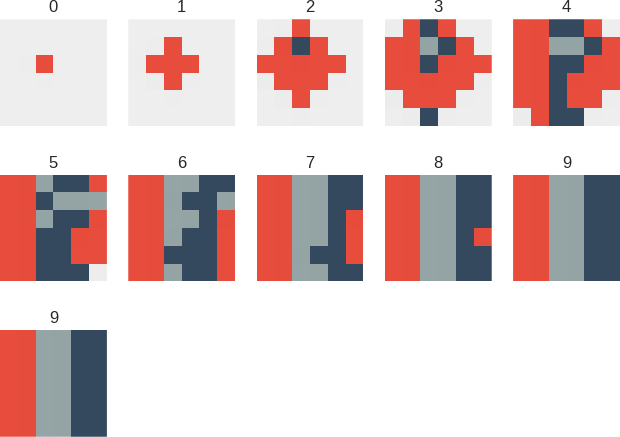
\includegraphics[width=\textwidth, keepaspectratio]{fig/result_figs/generate_tricolor/1}
\caption[A solution to the "Tricolor" morphogenesis]{A solution to the "Tricolor" morphogenesis that finds a point attractor equal to the target pattern.
Most solutions seen did not stabilize like this, but instead found a variety of cycles.}
\label{fig:tricolor_point_attractor}
\end{figure}

\begin{figure}
\centering
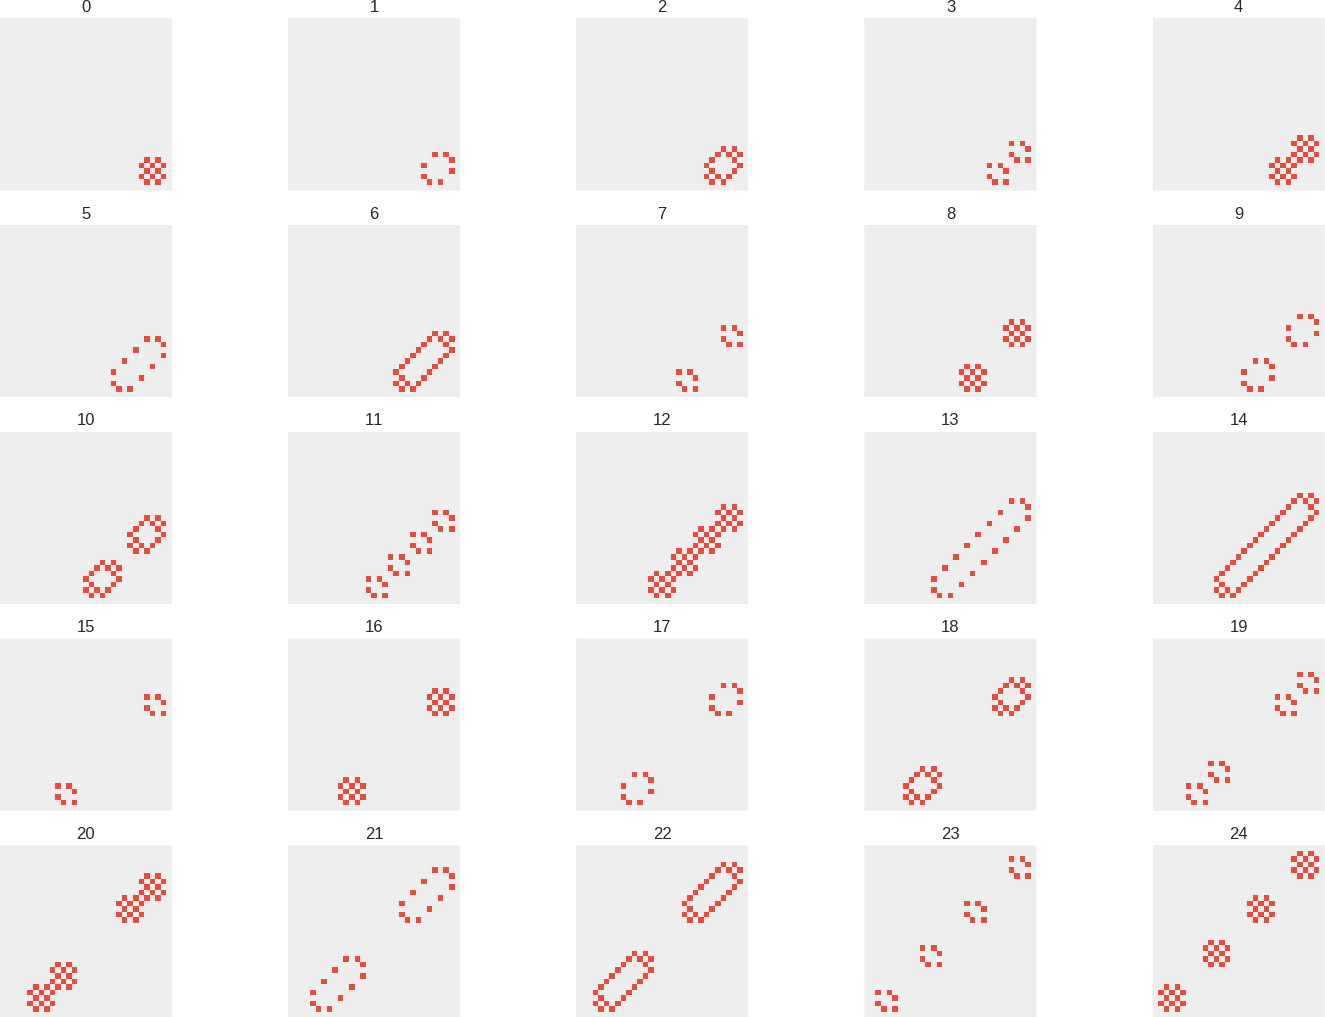
\includegraphics[width=\textwidth, keepaspectratio]{fig/result_figs/replicate_mosaic/7}
\caption[A solution to the "Mosaic" replication]{A solution to the "Mosaic" replication that shows multiple stages of replication.
First the original replicates into two copies. Then each copy tries to replicate, but they interfere with each other and instead return to one copy each, but at a greater distance.
Then they each succeed in replicating, producing four copies total.}
\label{fig:mosaic7}
\end{figure}

